%--- iliad ---
% title: "Reinforcement Learning"
% summary: >-
%   The Bellman equations and what follows from them: the existence of optimal
%   policies, the policy improvement theorem, the rate of convergence of
%   Bellman updates, and the convergence of Q-learning.
%--- end ---
\documentclass[11pt]{article}

% iliad.sty: local copy first (Overleaf), else the shared ../iliad.sty.
% Provides exercise/solution/definition/theorem/fact/callout and loads
% amsmath+amssymb+amsthm+enumitem+hyperref+cleveref.
\IfFileExists{iliad.sty}{\usepackage[boxes]{iliad}}{\usepackage[boxes]{../iliad}}

\usepackage{mathtools}
\usepackage{tikz}
\usetikzlibrary{positioning, arrows.meta}
% \llbracket/\rrbracket (Iverson brackets) come from iliad.sty — stmaryrd not needed.

\hypersetup{colorlinks=true, linkcolor=blue, urlcolor=blue, citecolor=blue}

% Math macros
\newcommand{\cS}{\mathcal{S}}
\newcommand{\cA}{\mathcal{A}}
\DeclareMathOperator*{\argmax}{arg\,max}

\title{Reinforcement Learning: Exercises}
\author{Leon Lang \and David Quarel}
\date{April 2026}

%===================================
\begin{document}
\maketitle

\begin{learningoutcomes}
  \begin{itemize}
    \item Understand Markov Decision Processes and the goal of the agent, for
      known environments.
    \item Understand the Bellman equation.
    \item Understand the policy improvement theorem, and how we can use it to
      iteratively solve for an optimal policy.
    \item Prove properties involving the Bellman equations, including the
      existence of optimal policies, the policy improvement theorem, rate of
      convergence of Bellman updates, and the convergence of Q-learning.
  \end{itemize}
\end{learningoutcomes}

%===================================

\section*{Setup}
In this exercise sheet, we prove a variety of results that are behind the \href{https://learn.arena.education/chapter2_rl/01_intro_rl/}{ARENA Intro to RL materials}. 
%Unlike the general (history-based) reinforcement learning setting, here we restrict attention to \textbf{Markov decision processes} (MDPs), where transitions and rewards depend only on the current state and action rather than on the full interaction history.

An \textbf{agent} interacts with an \textbf{environment} in discrete time steps $t = 0, 1, 2, \ldots$. On timestep $t$, the agent observes the current state $s_t \in \cS$ and selects an action $a_t \in \cA$ according to its policy. The environment then responds with a reward $r_{t+1} \in \mathbb{R}$ and a new state $s_{t+1} \in \cS$. (The reward and next state are indexed by $t+1$ because they are produced by the environment after the agent's action.) The goal is to act so as to maximize expected discounted future reward.

These environments are called \textbf{Markov decision processes} (MDPs). They satisfy two key properties: (i)~\textbf{stationarity} --- the transition and reward functions do not change over time, and (ii)~the \textbf{Markov property} --- the distribution over the next state and reward depends only on the current state and action, not on the full history of past interactions. Together, these properties mean that the current state $s_t$ is a sufficient summary of the past for the purpose of choosing optimal actions.

% ================================================

\begin{definition}[Spaces and notation]\label{def:spaces}\
\begin{itemize}\itemsep=2pt
    \item $\cS$ --- finite \textbf{state space}
    \item $\cA$ --- finite \textbf{action space}
    \item $\gamma \in (0, 1)$ --- \textbf{discount factor}
    \item $\Delta X$ --- set of all probability distributions over a set $X$
    \item $\llbracket P \rrbracket$ --- \textbf{Iverson bracket}: $1$ if $P$ is true, $0$ if false
\end{itemize}
\end{definition}

\begin{definition}[Environment]\label{def:environment}
An MDP \textbf{environment} is specified by a pair $(T, R)$:
\begin{itemize}\itemsep=2pt
    \item $T : \cS \times \cA \to \Delta \cS$ is the \textbf{transition kernel}: given state $s$ and action $a$, the next state is drawn $s' \sim T(\cdot \mid s, a)$.
    \item $R : \cS \times \cA \times \cS \to \mathbb{R}$ is the \textbf{reward function}: on a transition from $s$ to $s'$ under action $a$, the agent receives reward $R(s, a, s')$.
    \footnote{Noting that $\cS \times \cA \times \cS$ is a finite set, this implies that the rewards are bounded above by $R_\text{max} = \max_{s,a,s'} R(s,a,s')$.}
\end{itemize}
\end{definition}

\begin{definition}[Policy]\label{def:policy}
A \textbf{policy} $\pi : \cS \to \Delta \cA$ maps each state to a probability distribution over actions. Given state $s$:
\begin{itemize}\itemsep=2pt
    \item $\pi(\cdot \mid s)$ is a distribution over $\cA$,
    \item $\pi(a \mid s) \in [0, 1]$ is the probability of choosing action $a$,
    \item the agent samples $a \sim \pi(\cdot \mid s)$.
\end{itemize}
A policy is \textbf{deterministic} if $\pi(a \mid s) \in \{0, 1\}$ for all $a, s$. In this case, we abuse notation and write $\pi(s) := \argmax_{a \in \cA} \pi(a \mid s)$ for the unique action selected at state $s$.
\end{definition}

\begin{definition}[Trajectory]\label{def:trajectory}
When policy $\pi$ interacts with environment $(T, R)$ starting from initial state $s_0$, the resulting \textbf{trajectory} $(s_0, a_0, r_1, s_1, a_1, r_2, s_2, a_2, r_3, \ldots)$ is generated by
\[
    a_k \sim \pi(\cdot \mid s_k), \qquad s_{k+1} \sim T(\cdot \mid s_k, a_k), \qquad r_{k+1} = R(s_k, a_k, s_{k+1}),
\]
for $k = 0, 1, 2, \ldots$. We write $\mathbb{E}_\pi[\,\cdot\,]$ for expectations over such trajectories.
\end{definition}

% ================================================

\section{The Bellman equation}\label{prob:bellman}

\begin{definition}[Return]\label{def:return}
The \textbf{return} from time $t$ is the discounted sum of future rewards:
$$
G_t \;:=\; \sum_{k=t+1}^{\infty} \gamma^{k-t-1}\, r_k \;=\; r_{t+1} + \gamma\, r_{t+2} + \gamma^2\, r_{t+3} + \cdots.
$$
It satisfies the recursion
$$
G_t \;=\; r_{t+1} + \gamma\, G_{t+1}.
$$
\end{definition}

\begin{definition}[Value function]\label{def:value}
The \textbf{value function} of a policy $\pi$ is the expected return when starting from state $s$ and acting according to $\pi$:
\begin{align*}
&V_\pi(s) \;=\; \mathbb{E}_\pi\!\left[G_t \;\middle|\; s_t = s\right] \\
&=\; \mathbb{E}_\pi\!\left[\,r_{t+1} + \gamma\, r_{t+2} + \gamma^2\, r_{t+3} + \cdots \;\middle|\; s_t = s\right] \\
&=\; \sum_{a_t \in \cA} \pi(a_t \mid s)\! \sum_{s_{t+1} \in \cS} \!T(s_{t+1} \mid s, a_t)\! \sum_{a_{t+1} \in \cA} \pi(a_{t+1} \mid s_{t+1}) \\
&\quad \sum_{s_{t+2} \in \cS} \!T(s_{t+2} \mid s_{t+1}, a_{t+1})\, \cdots \\
&\quad \bigl[\, R(s, a_t, s_{t+1}) + \gamma\, R(s_{t+1}, a_{t+1}, s_{t+2}) + \gamma^2\, R(s_{t+2}, a_{t+2}, s_{t+3}) + \cdots \,\bigr].
\end{align*}
The expectation averages the return over all future trajectories $(a_t, s_{t+1}, a_{t+1}, s_{t+2}, \ldots)$ generated by sampling $a_k \sim \pi(\cdot \mid s_k)$ and $s_{k+1} \sim T(\cdot \mid s_k, a_k)$, starting from $s_t = s$.
\end{definition}

\begin{exercise}
\label{prob:bellman_proof} Prove the \textbf{Bellman equation}: for all $s \in \cS$,
\begin{callout}[note]
\textbf{Bellman Equation}
$$
V_\pi(s) = \sum_{a \in \cA} \pi(a \mid s) \sum_{s' \in \cS} T(s' \mid s, a)\bigl(R(s,a,s') + \gamma\, V_\pi(s')\bigr).
$$
\end{callout}
\textit{Hint:} condition on the first action and the first transition, then separate the immediate reward from the remaining return.
\end{exercise}


\begin{definition}[Action-value function]\label{def:q_function}
The \textbf{action-value function} (or Q-function) of $\pi$ is the expected return starting from state $s$, taking action $a$, and acting according to $\pi$ thereafter:
$$
Q_\pi(s,a) \;=\; \mathbb{E}_\pi\!\left[G_t \;\middle|\; s_t = s,\, a_t = a\right].
$$
\end{definition}

\begin{exercise}
\label{prob:q_function}
\begin{enumerate}
\item\label{prob:Vpi_from_Qpi} Express $V_\pi(s)$ in terms of $Q_\pi$.
\item\label{prob:Qpi_from_Vpi} Express $Q_\pi(s,a)$ in terms of $V_\pi$.
\item\label{prob:bellman_Q} Using these relations, derive a recursive equation for $Q_\pi$ analogous to the Bellman equation above.
\end{enumerate}
\end{exercise}


% ================================================

\section{An example MDP}\label{prob:small_mdp}

Consider the MDP with state space $\cS = \{s_0, s_L, s_R\}$, action space $\cA = \{a_L, a_R\}$, and deterministic transitions as shown:

\begin{center}
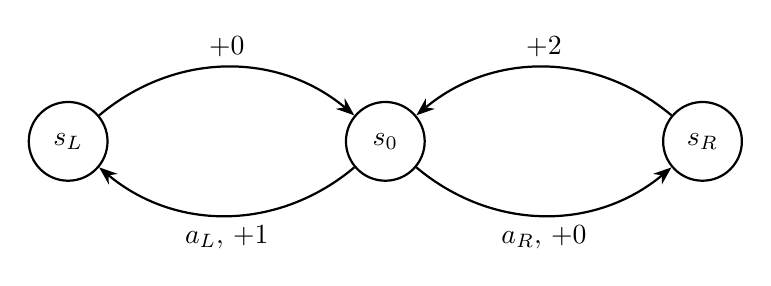
\begin{tikzpicture}[->, >=Stealth, thick, node distance=3cm,
    state/.style={circle, draw, minimum size=1cm, inner sep=2pt}]
  \node[state] (sL) {$s_L$};
  \node[state] (s0) [right=of sL] {$s_0$};
  \node[state] (sR) [right=of s0] {$s_R$};
  \draw (s0) to[bend left=40]  node[midway, below] {$a_L,\,+1$} (sL);
  \draw (sL) to[bend left=40]  node[midway, above] {$+0$}       (s0);
  \draw (s0) to[bend right=40] node[midway, below] {$a_R,\,+0$} (sR);
  \draw (sR) to[bend right=40] node[midway, above] {$+2$}       (s0);
\end{tikzpicture}
\end{center}

From $s_0$, action $a_L$ leads deterministically to $s_L$ with reward $+1$, and action $a_R$ leads deterministically to $s_R$ with reward $+0$. From $s_L$ (resp.\ $s_R$), any action returns to $s_0$ with reward $+0$ (resp.\ $+2$).

Let $\pi_L$ denote the policy that always selects $a_L$, and $\pi_R$ the policy that always selects $a_R$.

\begin{exercise}
\label{prob:small_mdp_values} Using the Bellman equation from \cref{prob:bellman_proof}, verify that
$$
V_{\pi_L}(s_0) = \frac{1}{1-\gamma^2}, \qquad V_{\pi_R}(s_0) = \frac{2\gamma}{1-\gamma^2}.
$$
\end{exercise}


\begin{exercise}
\label{prob:small_mdp_optimal} Determine the best action from state $s_0$ as a function of the discount factor $\gamma \in (0, 1)$. Show that the breakeven point is $\gamma = \tfrac{1}{2}$.
\end{exercise}

% ================================================

\section{Bellman operators and the existence of optimal policies}\label{prob:bellman_ops}

\subsection*{Banach fixed-point theorem}

In this and the following exercises, we will make use of the well-known Banach fixed point theorem:

\begin{theorem}[Banach Fixed Point Theorem]\label{thm:banach}
Let $(X, d)$ be a complete metric space and let $F : X \to X$ be a contraction mapping, i.e.\ there exists $\gamma \in [0,1)$ such that
$$
d(F(x), F(y)) \le \gamma\, d(x, y) \quad \text{for all } x, y \in X.
$$
Then $F$ has a unique fixed point $x^* \in X$ satisfying $F(x^*) = x^*$. Moreover, for any initial point $x_0 \in X$, one 
%has $F^n(x_0) \to x^*$ as $n \to \infty$, 
has $\lim_{n \to \infty} d(F^n(x_0), x^*) = 0$ 
where $F^n$ is the $n$-fold composition of $F$ with itself. That is, $F^n(x_0)$ converges to $x^*$ with respect to the metric $d$.
\end{theorem}

\subsection*{The problem}

\begin{definition}[Bellman optimality operator]\label{def:bellman_op}
Let $\mathcal{V} = \{V : \cS \to \mathbb{R}\}$ denote the vector space of value functions, equipped with the sup-norm
$\|V\|_\infty = \max_{s \in \cS} |V(s)|$.
The \textbf{Bellman optimality operator} $\mathcal{B} : \mathcal{V} \to \mathcal{V}$ is defined by
$$
(\mathcal{B} V)(s) \coloneqq \max_{a \in \cA} \sum_{s' \in \cS} T(s' \mid s, a)\bigl(R(s,a,s') + \gamma\, V(s')\bigr).
$$
\end{definition}

\begin{exercise}
\label{prob:max_ineq} Let $f, g : \cA \to \mathbb{R}$ be real-valued functions on a finite set $\cA$. Prove that
$$
\left|\max_{a \in \cA} f(a) - \max_{a \in \cA} g(a)\right| \le \max_{a \in \cA} |f(a) - g(a)|.
$$
\end{exercise}


\begin{exercise}
\label{prob:B_contraction} Using \cref{prob:max_ineq}, prove that $\mathcal{B}$ is a \textbf{contraction mapping} with contraction factor $\gamma$, i.e.\ for all $V, W \in \mathcal{V}$,
$$
\|\mathcal{B} V - \mathcal{B} W\|_\infty \le \gamma\, \|V - W\|_\infty.
$$
\end{exercise}


\begin{exercise}
\label{prob:V_star_exists} Using \cref{thm:banach}, conclude that there exists a unique $V^* \in \mathcal{V}$ satisfying $\mathcal{B} V^* = V^*$, and that for any initial $V_0 \in \mathcal{V}$, the iterates $\mathcal{B}^n V_0 \to V^*$ as $n \to \infty$.
\end{exercise}


\begin{exercise}
\label{prob:Bpi_contraction} Show that for any policy $\pi$, the operator $\mathcal{B}_\pi : \mathcal{V} \to \mathcal{V}$ defined by
\begin{callout}[note]
\textbf{Bellman Policy Operator}
$$
(\mathcal{B}_\pi V)(s) \coloneqq \sum_{a \in \cA} \pi(a \mid s) \sum_{s' \in \cS} T(s' \mid s, a)\bigl(R(s,a,s') + \gamma\, V(s')\bigr)
$$
\end{callout}
is also a contraction with factor $\gamma$. Conclude that $V_\pi$ is its unique fixed point and that $\mathcal{B}^n_{\pi} V_0 \to V_{\pi}$ for any initial $V_0 \in \mathcal{V}$ as $n \to \infty$.

\emph{Remark.} This shows that the numerical policy evaluation algorithm from the ARENA materials converges to the correct solution.
\end{exercise}


% ================================================

\begin{exercise}
\label{prob:greedy_equals_B} Let $V \in \mathcal{V}$ be any value function, and let $\pi_V$ be a greedy policy with respect to $V$, i.e.\
$$
\pi_V(s) \in \argmax_{a \in \cA} \sum_{s' \in \cS} T(s' \mid s, a)\bigl(R(s,a,s') + \gamma\, V(s')\bigr).
$$
Show that $\mathcal{B}_{\pi_V} V = \mathcal{B} V$.
\end{exercise}


\begin{exercise}
\label{prob:V_pi_star} Define the \textbf{greedy policy} with respect to $V^*$ by $\pi^* = \pi_{V^*}$ as in the previous part.
Show that $V_{\pi^*} = V^*$, i.e.\ the value function of $\pi^*$ equals the fixed point of $\mathcal{B}$.

\textit{Hint:} show that $V^*$ satisfies the same fixed-point equation as $V_{\pi^*}$.
\end{exercise}


\begin{exercise}
\label{prob:optimality} Conclude that $\pi^*$ is an \textbf{optimal policy}: for every policy $\pi$ and every state $s \in \cS$,
$$
V_{\pi^*}(s) \ge V_\pi(s).
$$
\textit{Hint:} show that $\mathcal{B} V_\pi \ge V_\pi$ pointwise, then iterate and take the limit.
\end{exercise}


% ================================================


\section{Policy improvement theorem}\label{prob:policy_improvement}

Given a policy $\pi$, define the \textbf{improved policy} $\pi'$ greedily with respect to $V_\pi$:

\begin{callout}[note]
\textbf{Policy Improvement}
$$
\pi'(s) \in \argmax_{a \in \cA} \sum_{s' \in \cS} T(s' \mid s, a)\bigl(R(s,a,s') + \gamma\, V_\pi(s')\bigr).
$$
\end{callout}

\begin{exercise}
\label{prob:when_equality} In proving \cref{prob:optimality}, we already saw that for all $s \in \cS$, we have
$(\mathcal{B} V_\pi)(s) \ge V_\pi(s)$.
When does equality hold for all states?
\end{exercise}


\begin{exercise}
\label{prob:policy_improvement_thm} Show that $V_{\pi'}(s) \ge V_\pi(s)$ for all $s \in \cS$.

\textit{Hint:} show that $\mathcal{B}_{\pi'} V_\pi \ge V_\pi$ pointwise using \cref{prob:greedy_equals_B}, then iterate $\mathcal{B}_{\pi'}$ and take the limit.
\end{exercise}


\begin{exercise}
\label{prob:policy_iteration} The \textbf{policy iteration} algorithm generates a sequence of policies $\pi_0, \pi_1, \pi_2, \ldots$ where each $\pi_{k+1}$ is the greedy policy with respect to $V_{\pi_k}$. Show that this sequence converges to an optimal policy $\pi^*$ in a finite number of steps.

\textit{Hint:} how many deterministic policies are there?
\end{exercise}



% ============================================


\section{Bellman convergence rate}\label{prob:convergence_rate}

\Cref{prob:V_star_exists} showed that the iterates $V_n := \mathcal{B}^n V_0$ converge to $V^*$ for any starting $V_0 \in \mathcal{V}$, but it did not tell us \emph{how fast}, nor how to decide when to stop iterating. We derive some convergence rate bounds \cite[Chapter~6]{putermanMarkovDecisionProcesses1994}.

\begin{exercise}
\label{prob:geometric_decay} Show that for any initial $V_0 \in \mathcal{V}$, the iterates $V_n := \mathcal{B}^n V_0$ satisfy
$$
\|V_n - V^*\|_\infty \;\le\; \gamma^n \|V_0 - V^*\|_\infty.
$$
\emph{Remark.} This bound is not useful as a stopping criterion in practice as it depends on the unknown $V^*$.
\end{exercise}


\begin{exercise}
\label{prob:a_priori_bound} Show the \textbf{a~priori bound}:
$$
\|V_n - V^*\|_\infty \;\le\; \frac{\gamma^n}{1-\gamma}\, \|V_1 - V_0\|_\infty.
$$
This bound uses only $\|V_1 - V_0\|_\infty$ --- a quantity computable after a single iteration, independent of $V^*$.

\textit{Hint:} write $V^* - V_n = \sum_{k=n}^{\infty}(V_{k+1} - V_k)$ (valid since $V_k \to V^*$), and bound each term using the contraction of $\mathcal{B}$.
\end{exercise}


\begin{exercise}
\label{prob:a_posteriori_bound} Show the \textbf{a~posteriori bound}: for $n \ge 1$,
$$
\|V_n - V^*\|_\infty \;\le\; \frac{\gamma}{1-\gamma}\, \|V_n - V_{n-1}\|_\infty.
$$

\textit{Hint:} telescope from $n$ as in \cref{prob:a_priori_bound}, but bound $\|V_{k+1} - V_k\|_\infty$ in terms of $\|V_n - V_{n-1}\|_\infty$ instead.
\end{exercise}


\begin{exercise}
\label{prob:a_posteriori_tighter} Show that the a~posteriori bound of \cref{prob:a_posteriori_bound} is always at least as tight as the a~priori bound of \cref{prob:a_priori_bound}: for all $n \ge 1$,
$$
\frac{\gamma}{1-\gamma}\, \|V_n - V_{n-1}\|_\infty \;\le\; \frac{\gamma^n}{1-\gamma}\, \|V_1 - V_0\|_\infty.
$$

\textit{Hint:} bound $\|V_n - V_{n-1}\|_\infty$ by repeated application of the contraction.
\end{exercise}


\begin{exercise}
\label{prob:concrete_bound} Assume $|R(s,a,s')| \le R_{\max}$ for all $s,a,s'$. Show that if we initialize with $V_0 \equiv 0$, then
$$
\|V_n - V^*\|_\infty \;\le\; \frac{\gamma^n}{1-\gamma}\, R_{\max}.
$$
This bound depends only on $n$, $\gamma$, and $R_{\max}$, so it can be evaluated before running a single iteration.
\end{exercise}


\begin{exercise}
\label{prob:bound_tight} Show that the bound of \cref{prob:concrete_bound} is \textbf{tight}: exhibit an MDP in which $\|V_n - V^*\|_\infty = \frac{\gamma^n}{1-\gamma}\, R_{\max}$ for every $n \ge 0$ (with $V_0 \equiv 0$).
%\textit{Hint:} consider the single-state, single-action MDP that always returns reward $R_{\max}$.}
\end{exercise}


% \mysubsection{6}{\label{prob:iteration_count} Given a desired error tolerance $\delta > 0$, show that under the assumptions of \cref{prob:concrete_bound} (i.e., $V_0 \equiv 0$ and $|R(s,a,s')| \le R_{\max}$), guaranteeing $\|V_n - V^*\|_\infty \le \delta$ via the bound of \cref{prob:concrete_bound} requires
% $$
% n \;\ge\; \frac{\log\!\dfrac{R_{\max}}{\delta(1-\gamma)}}{\log(1/\gamma)}.
% $$
% By \cref{prob:bound_tight}, this threshold cannot be improved using only $(\gamma, R_{\max})$ information.}

% \begin{solution}
% Start from the bound of \cref{prob:concrete_bound} and require its right-hand side to be at most $\delta$:
% $$
% \frac{\gamma^n}{1-\gamma}\, R_{\max} \;\le\; \delta
% \qquad\Longleftrightarrow\qquad
% \gamma^n \;\le\; \frac{\delta(1-\gamma)}{R_{\max}}.
% $$
% Taking the logarithm of both sides and noting $\log \gamma < 0$ (since $\gamma \in (0, 1)$), the inequality flips upon dividing by $\log \gamma$:
% $$
% n \;\ge\; \frac{\log\!\dfrac{\delta(1-\gamma)}{R_{\max}}}{\log \gamma}
% \;=\; \frac{-\log\!\dfrac{\delta(1-\gamma)}{R_{\max}}}{-\log\gamma}
% \;=\; \frac{\log\!\dfrac{R_{\max}}{\delta(1-\gamma)}}{\log(1/\gamma)}.
% $$
% For tightness: on the MDP of \cref{prob:bound_tight} we have equality $\|V_n - V^*\|_\infty = \frac{\gamma^n}{1-\gamma}R_{\max}$, so any $n$ strictly below this threshold yields error strictly greater than $\delta$.
% \end{solution}

% \mysubsection{7}{\label{prob:iteration_count_clean} The bound of \cref{prob:iteration_count} has $\log(1/\gamma)$ in the denominator, which obscures its scaling in $\gamma$. Derive a slightly weaker but more transparent sufficient condition:
% $$
% n \;\ge\; \frac{1}{1-\gamma}\log\!\frac{R_{\max}}{\delta(1-\gamma)} \;\;\Longrightarrow\;\; \|V_n - V^*\|_\infty \le \delta.
% $$

% \textit{Hint:} show that $\log(1/\gamma) \ge 1-\gamma$ for all $\gamma \in (0, 1)$. This approximation is very tight when $\gamma$ is close to $1$, since $\log(1/\gamma) = (1-\gamma) + O\bigl((1-\gamma)^2\bigr)$.}

% \begin{solution}
% Let $x := 1 - \gamma \in (0, 1)$, so $\log(1/\gamma) = -\log(1 - x)$. The Taylor expansion around $x = 0$ gives
% $$
% -\log(1 - x) \;=\; x + \frac{x^2}{2} + \frac{x^3}{3} + \cdots \;\ge\; x
% $$
% for all $x \in (0, 1)$ (all higher-order terms are nonnegative), i.e.\ $\log(1/\gamma) \ge 1-\gamma$. As $\gamma \to 1^-$, the higher-order terms vanish and $\log(1/\gamma) \to (1-\gamma)$, so the inequality is asymptotically tight.

% Applying this to \cref{prob:iteration_count}: since $\log(1/\gamma) \ge 1-\gamma > 0$ and the numerator $\log\!\dfrac{R_{\max}}{\delta(1-\gamma)} > 0$ (assuming $\delta < \dfrac{R_{\max}}{1-\gamma}$, which is the interesting regime),
% $$
% \frac{\log\!\dfrac{R_{\max}}{\delta(1-\gamma)}}{\log(1/\gamma)}
% \;\le\; \frac{1}{1-\gamma}\log\!\frac{R_{\max}}{\delta(1-\gamma)}.
% $$
% Hence any $n$ satisfying the latter also satisfies the exact threshold of \cref{prob:iteration_count}, and therefore guarantees $\|V_n - V^*\|_\infty \le \delta$.
% \end{solution}

% \emph{Remark.} Splitting the log:
% $$
% n \;\ge\; \frac{1}{1-\gamma}\!\left[\log\!\frac{1}{\delta} \;+\; \log\!\frac{R_{\max}}{1-\gamma}\right].
% $$
% The dependence on $\delta$ is \emph{only} through $\log(1/\delta)$: halving $\delta$ (doubling precision) costs a constant $\frac{\log 2}{1-\gamma} \approx \frac{0.7}{1-\gamma}$ extra iterations, regardless of how small $\delta$ already is. This is geometric convergence: each iteration buys a fixed multiplicative improvement in the error. The expensive part of the bound is the $\frac{1}{1-\gamma}$ prefactor --- the \textbf{effective horizon} --- which blows up as $\gamma \to 1$. So the true cost driver is $\gamma$ near $1$, not $\delta$ near $0$.

\emph{Remark.} Combining \cref{prob:a_posteriori_bound,prob:a_priori_bound,prob:concrete_bound} gives a chain of progressively weaker but increasingly upfront-computable bounds:

\begin{callout}[note]
\textbf{Convergence Bounds}
\begin{align*}
\|V_n - V^*\|_\infty
\;&\le\; \underbrace{\tfrac{\gamma}{1-\gamma}\, \|V_n - V_{n-1}\|_\infty}_{\text{a~posteriori, tightest}}
\;\le\; \underbrace{\tfrac{\gamma^n}{1-\gamma}\, \|V_1 - V_0\|_\infty}_{\text{a~priori}} \\
\;&\le\; \underbrace{\tfrac{\gamma^n}{1-\gamma}\, R_{\max}}_{\text{upfront, assumes } V_0 \equiv 0,\, |R| \le R_{\max}}.
\end{align*}
\end{callout}
Each step weakens the bound by replacing realized information with something coarser: first the most recent step size $\|V_n - V_{n-1}\|_\infty$ with the worst-case geometric decay $\gamma^{n-1}\|V_1 - V_0\|_\infty$ (contraction of $\mathcal{B}$ applied $n-1$ times), then the initial step size $\|V_1 - V_0\|_\infty$ with the crude reward bound $R_{\max}$. In practice the leftmost bound is significantly tighter, since $\|V_n - V_{n-1}\|_\infty$ often decays strictly faster than $\gamma^{n-1}\|V_1 - V_0\|_\infty$. It also yields a concrete stopping rule: to guarantee $\|V_n - V^*\|_\infty \le \varepsilon$, iterate until $\|V_n - V_{n-1}\|_\infty \le \frac{1-\gamma}{\gamma}\, \varepsilon$.

% The useless bound of \cref{prob:geometric_decay}, $\|V_n - V^*\|_\infty \le \gamma^n \|V_0 - V^*\|_\infty$, does not belong to this chain: its right-hand side itself requires bounding via $\|V_0 - V^*\|_\infty \le \tfrac{1}{1-\gamma}\|V_1 - V_0\|_\infty$ (from \cref{prob:a_priori_bound} with $n = 0$) before it becomes computable, and that substitution recovers the a~priori bound exactly.

% ============================================

\section{Convergence of Q-learning}\label{prob:q_learning}

The policy improvement theorem from \cref{prob:policy_improvement} shows that we can in principle find an optimal policy in MDPs. However, it makes the uncomfortable assumption that we know the environment dynamics via the transition kernel $T$. In this problem, we prove that $Q$-learning, which does not make such an assumption, converges to the optimal action-value function, from which one can trivially extract an optimal policy by choosing actions greedily.

\subsection*{Stochastic approximation theorem}

We will make use of the following stochastic approximation result, which we state without proof:

\begin{theorem}[Stochastic Approximation for Contractions {\cite[Theorem~3]{tsitsiklis1994}}]\label{thm:stochastic_approx}
Let $\mathcal{X} = \{x : I \to \mathbb{R}\}$ be the space of real-valued functions on a finite set $I$, equipped with the sup-norm $\|x\|_\infty = \max_i |x(i)|$. Let $F : \mathcal{X} \to \mathcal{X}$ be a contraction mapping with factor $\gamma \in [0,1)$ and unique fixed point $x^*$.

Fix an initial iterate $x_0 \in \mathcal{X}$, and for each $t \geq 0$ let $\alpha_t : I \to [0,1]$ be a \textbf{learning rate} function and $w_t : I \to \mathbb{R}$ a random \textbf{noise} function (both functions on $I$, one value per coordinate). Consider the stochastic iteration
$$
x_{t+1}(i) = (1 - \alpha_t(i))\, x_t(i) + \alpha_t(i)\bigl[F(x_t)(i) + w_t(i)\bigr] \qquad \text{for all } i \in I,
$$
where updates are applied to a single coordinate $i = i_t$ at each step (i.e.\ $\alpha_t(i) = 0$ for $i \neq i_t$). Suppose:
\begin{enumerate}
\item[(a)] \textbf{(Learning rate)} For each $i \in I$:
$$
\sum_{t=0}^{\infty} \alpha_t(i) = \infty, \qquad \sum_{t=0}^{\infty} \alpha_t(i)^2 < \infty, \qquad \alpha_t(i) \in [0,1].
$$
\item[(b)] \textbf{(Noise)} For each $i \in I$, conditioned on the history $\mathcal{F}_t = \{x_0, \alpha_0, w_0, \alpha_1, w_1, \ldots, \alpha_{t-1}, w_{t-1}, x_t, \alpha_t\}$, the noise has zero mean and bounded variance:
$$
\mathbb{E}\big[w_t(i) \mid \mathcal{F}_t\big] = 0, \qquad \mathbb{E}\big[w_t(i)^2 \mid \mathcal{F}_t\big] \le C\bigl(1 + \|x_t\|_\infty^2\bigr)
$$
for some constant $C > 0$.
\end{enumerate}
Then $x_t(i) \to x^*(i)$ for all $i \in I$, with probability $1$.
\end{theorem}

\emph{What is stochastic?}
The randomness of the iteration is carried by the noise: each $w_t(i)$ is a real-valued random variable, and $w_t$ is a random element of $\mathbb{R}^I$. Consequently, the iterates $x_1, x_2, \ldots$ are random (they depend on past noise $w_0, \ldots, w_{t-1}$), and the learning rates $\alpha_t(i)$ may be random as well if they depend on the history---e.g.\ on which coordinate was just visited. The contraction $F$, its fixed point $x^*$, the update rule itself, and the initial iterate $x_0$ are all deterministic. The theorem asserts that despite the noise, the random sequence $(x_t)$ converges pointwise to $x^*$ almost surely.

\emph{Remark on ``with probability $1$''.}
The conclusion $x_t(i) \to x^*(i)$ with probability $1$ (also called \textbf{almost sure convergence}) means
$$
P\!\left(\lim_{t \to \infty} x_t(i) = x^*(i)\right) = 1 \quad \text{for all } i \in I.
$$
In other words, the probability that a run of the stochastic iteration fails to converge to $x^*$ is zero.

% TODO: Better place to put this? Or scrap it all-together?
% \emph{Why ``almost surely'' and not ``surely''?}
% The phrase ``with probability $1$'' is subtly different from ``for every possible sequence of outcomes.'' To see why the distinction matters, consider a simpler estimation problem: learning the bias of a coin.

% Suppose a coin lands heads with probability $p = 1/3$ and tails with probability $2/3$. We flip it repeatedly and track the running fraction of heads. The strong law of large numbers guarantees this fraction converges to $1/3$ \emph{almost surely}: for all infinite sequences of outcomes except a set of probability zero.

% Which sequences fail? Consider $\omega = (H, H, H, H, \ldots)$ --- heads on every single flip. If we only observed this sequence, we would estimate $p = 1$ instead of $p = 1/3$. This sequence is logically possible (each individual flip can land heads), but its probability under the true distribution is
% $$
% P(\omega) = \prod_{k=1}^{\infty} \frac{1}{3} = \lim_{n \to \infty} \left(\frac{1}{3}\right)^n = 0.
% $$
% Convergence holds for all sequences \emph{except} a set of such measure-zero pathologies. This is precisely what ``almost sure'' convergence means.

% The same phenomenon occurs in Q-learning. \Cref{thm:stochastic_approx} guarantees $Q_t \to Q^*$ almost surely: there exist pathological sequences of transitions under which Q-learning would fail to converge (e.g., if the environment happened to produce the same next-state on every single visit to some state-action pair, forever), but the set of all such sequences has probability zero under the true transition kernel.

\emph{Why should we believe this?}
It helps to build up the result in three layers of increasing complexity.

\textbf{Layer 1: no noise, all coordinates at once.}
If $w_t = 0$ and $\alpha_t(i) = 1$ for all $i$ and $t$, the iteration reduces to $x_{t+1} = F(x_t)$. This converges to $x^*$ by \cref{thm:banach}.

\textbf{Layer 2: noise, but all coordinates at once.}
Now suppose we observe $F(x_t) + w_t$ instead of $F(x_t)$, and use a decreasing step size:
$$
x_{t+1} = (1 - \alpha_t)\,x_t + \alpha_t\bigl[F(x_t) + w_t\bigr] = x_t + \alpha_t\bigl[\underbrace{F(x_t) - x_t}_{\text{signal}} + \underbrace{w_t}_{\text{noise}}\bigr].
$$
The signal $F(x_t) - x_t$ always points toward $x^*$ (this is what the contraction property buys us). The noise $w_t$ is mean-zero, so it pushes us in random directions that partially cancel over time. The two conditions on the step size mediate between signal and noise:
\begin{itemize}
\item $\sum \alpha_t = \infty$ ensures the total step size is large enough to reach $x^*$ from any starting point.
\item $\sum \alpha_t^2 < \infty$ ensures the noise averages out. Each noise term $w_t$ enters the iteration scaled by $\alpha_t$, contributing a random displacement of size $\alpha_t w_t$. Although these displacements are not independent (each depends on the current iterate $x_t$), they are mean-zero conditioned on the past. For such sequences, the variance of the cumulative sum is the sum of the individual variances, which is proportional to $\sum \alpha_t^2$. Since this is finite, the total random drift converges and cannot overwhelm the steady pull of the signal toward~$x^*$.
\end{itemize}
The signal accumulates coherently (always pulling toward $x^*$), while the noise averages out.

\textbf{Layer 3: one coordinate at a time.}
The iteration updates only one coordinate $i = i_t$ per step, while the others stay frozen. This makes the analysis more difficult since the target $F(x_t)(i)$ depends on all coordinates, including stale ones. The condition $\sum_t \alpha_t(i) = \infty$ for each $i$ ensures no coordinate is permanently neglected, and the contraction property of $F$ provides enough global coupling to prevent coordinates from drifting apart. Making this rigorous is the main technical content of the proof.

\subsection*{The problem}

Consider the following generalization of the Q-learning update from the ARENA materials, now with a time-varying learning rate $\alpha_t > 0$: given a current estimate $Q_t : \cS \times \cA \to \mathbb{R}$ and an observed transition $(s_t, a_t, r_{t+1}, s_{t+1})$ where $s_{t+1} \sim T(\cdot \mid s_t, a_t)$ and $r_{t+1} = R(s_t, a_t, s_{t+1})$, the update is

\begin{callout}[note]
\textbf{Q-Learning Update}
$$
Q_{t+1}(s_t, a_t) = Q_t(s_t, a_t) + \alpha_t\bigl(r_{t+1} + \gamma \max_{a' \in \cA} Q_t(s_{t+1}, a') - Q_t(s_t, a_t)\bigr),
$$
\end{callout}
with $Q_{t+1}(s,a) = Q_t(s,a)$ for all $(s,a) \neq (s_t, a_t)$.
We will show that, under appropriate conditions, Q-learning converges to the optimal action-value function $Q^*$.

Let $\mathcal{Q} = \{Q : \cS \times \cA \to \mathbb{R}\}$ denote the space of action-value functions, equipped with the sup-norm $\|Q\|_\infty = \max_{s,a} |Q(s,a)|$.

\begin{exercise}
\label{prob:BQ_contraction} Overloading the notation from \cref{def:bellman_op}, define the \textbf{Bellman optimality operator} on action-value functions, $\mathcal{B} : \mathcal{Q} \to \mathcal{Q}$, by
\begin{callout}[note]
\textbf{Bellman Q-Operator}
$$
(\mathcal{B}Q)(s,a) \coloneqq \sum_{s' \in \cS} T(s' \mid s, a)\bigl[R(s,a,s') + \gamma \max_{a' \in \cA} Q(s', a')\bigr].
$$
\end{callout}
(Here $\mathcal{B}$ takes a $Q$-function to a $Q$-function, whereas the earlier $\mathcal{B}$ in \cref{def:bellman_op} takes a $V$-function to a $V$-function --- whether $\mathcal{B}$ denotes the $V$- or $Q$-version is always clear from its argument.) Show that $\mathcal{B}$ is a $\gamma$-contraction on $(\mathcal{Q}, \|\cdot\|_\infty)$.

\textit{Hint:} this is similar to the proof of \cref{prob:B_contraction}.
\end{exercise}


\begin{exercise}
\label{prob:bellman_opt_Q} Define $Q^* \coloneqq Q_{\pi^*}$, the action-value function of the optimal policy $\pi^*$ from \cref{prob:bellman_ops}. We now show Bellman optimality equations and their consequences.
\begin{enumerate}
\item\label{prob:Q_star_formula} Show that $Q^*(s,a) = \sum_{s' \in \cS} T(s' \mid s, a)\bigl[R(s,a,s') + \gamma\, V^*(s')\bigr]$.
\item\label{prob:V_star_max_Q} Show that $V^*(s) = \max_{a \in \cA} Q^*(s,a)$.
\item\label{prob:Q_star_fixed_point} Conclude that $Q^*$ is the unique fixed point of $\mathcal{B}$.
\end{enumerate}
\end{exercise}


\begin{exercise}
\label{prob:identify_SA} Rewrite the Q-learning update in the form of \cref{thm:stochastic_approx}:
$$
x_{t+1}(i) = (1 - \alpha_t(i))\, x_t(i) + \alpha_t(i)\bigl[F(x_t)(i) + w_t(i)\bigr].
$$
Specifically, identify the index set $I$, the mapping $F$, the iterates $x_t$, and the learning rates $\alpha_t(i)$. Then give an explicit expression for the noise $w_t$.
\end{exercise}


\begin{exercise}
\label{prob:noise_zero_mean} Show that the noise satisfies $\mathbb{E}[w_t(s,a) \mid \mathcal{F}_t] = 0$ for all $(s,a) \in \cS \times \cA$, where $\mathcal{F}_t$ denotes the history up to time $t$ as in \cref{thm:stochastic_approx}.

\textit{Hint:} conditioned on $\mathcal{F}_t$, the quantities $Q_t$, $s_t$, and $a_t$ are all determined. What is the only remaining source of randomness?
\end{exercise}


\begin{exercise}
\label{prob:noise_bounded_var} Assume $|R(s,a,s')| \le R_{\max}$ for all $s, a, s'$. Show that there exists a constant $C > 0$ (depending only on $R_{\max}$ and $\gamma$) such that
$$
\mathbb{E}\bigl[w_t(s,a)^2 \mid \mathcal{F}_t\bigr] \le C\bigl(1 + \|Q_t\|_\infty^2\bigr).
$$
\textit{Hint:} first show that $|w_t(s_t, a_t)| \le 2(R_{\max} + \gamma\, \|Q_t\|_\infty)$.
\end{exercise}


\begin{exercise}
\label{prob:q_learning_converge} Conclude: state the conditions on the learning rate schedule and the exploration policy under which Q-learning converges, i.e.\ $Q_t \to Q^*$ with probability $1$.
\emph{Remark.} The ARENA implementation uses a constant learning rate $\alpha$, which does not satisfy $\sum_t \alpha_t(s,a)^2 < \infty$. In practice, constant-rate Q-learning does not converge exactly but oscillates in a neighbourhood of $Q^*$ whose size shrinks with $\alpha$.
\end{exercise}



% ================================================

\section{Exact policy evaluation}\label{prob:exact_eval}

In \cref{prob:Bpi_contraction}, we showed that iterating $\mathcal{B}_\pi$ converges to $V_\pi$; this is the numerical policy evaluation scheme used in the ARENA materials. When the state space is finite and the dynamics $(T, R)$ are known, there is also an \emph{exact} (closed-form) solution: the Bellman equation becomes a linear system that can be solved directly. In this problem we derive that closed form for deterministic policies.

\begin{definition}[Matrix-vector notation for a deterministic policy]\label{def:matrix_notation}
Fix a deterministic policy $\pi$. Treating the value function as a vector in $\mathbb{R}^{|\cS|}$, define:
\begin{itemize}\itemsep=2pt
  \item $\mathbf{v}^\pi \in \mathbb{R}^{|\cS|}$ with $\mathbf{v}^\pi_s := V_\pi(s)$,
  \item $\mathbf{P}^\pi \in \mathbb{R}^{|\cS| \times |\cS|}$ with $\mathbf{P}^\pi_{s,s'} := T(s' \mid s, \pi(s))$ (the \textbf{transition matrix} under $\pi$),
  \item $\mathbf{R}^\pi \in \mathbb{R}^{|\cS| \times |\cS|}$ with $\mathbf{R}^\pi_{s,s'} := R(s, \pi(s), s')$ (the \textbf{reward matrix}),
  \item $\mathbf{r}^\pi \in \mathbb{R}^{|\cS|}$ with $\mathbf{r}^\pi_s := \sum_{s'} \mathbf{P}^\pi_{s,s'}\, \mathbf{R}^\pi_{s,s'} = \sum_{s'} T(s' \mid s, \pi(s))\, R(s, \pi(s), s')$ (the \textbf{expected immediate reward}).
\end{itemize}
\end{definition}

\begin{fact}[Neumann series]\label{fact:neumann}
Equip $\mathbb{R}^{n \times n}$ with the induced $\infty$-norm
$$\|\mathbf{A}\|_\infty \;:=\; \max_i \sum_j |\mathbf{A}_{ij}| \qquad \text{(maximum absolute row sum).}$$
If $\|\mathbf{A}\|_\infty < 1$, then $\mathbf{I} - \mathbf{A}$ is invertible, and
$$(\mathbf{I} - \mathbf{A})^{-1} \;=\; \sum_{k=0}^{\infty} \mathbf{A}^k.$$
\end{fact}

\begin{exercise}
\label{prob:exact_eval_derive} Starting from the Bellman equation (\cref{prob:bellman_proof}) applied to a deterministic policy $\pi$, show that
\begin{callout}[note]
\textbf{Exact Policy Evaluation}
$$
\mathbf{v}^\pi \;=\; (\mathbf{I} - \gamma\, \mathbf{P}^\pi)^{-1}\, \mathbf{r}^\pi,
$$
\end{callout}
assuming $\mathbf{I} - \gamma\, \mathbf{P}^\pi$ is invertible (which we prove in \cref{prob:exact_eval_invertible}).

\textit{Hint:} specialize the Bellman equation to a deterministic policy and write the resulting system of $|\cS|$ equations in matrix-vector form.
\end{exercise}


\begin{exercise}
\label{prob:exact_eval_invertible} Prove that $\mathbf{I} - \gamma\, \mathbf{P}^\pi$ is invertible for any deterministic policy $\pi$ and any $\gamma \in (0, 1)$.

\textit{Hint:} apply \cref{fact:neumann}.
\end{exercise}


\emph{Remark.} The same derivation extends to stochastic policies by defining $\mathbf{P}^\pi_{s,s'} = \sum_{a} \pi(a \mid s)\, T(s' \mid s, a)$ and $\mathbf{r}^\pi_s = \sum_{a} \pi(a \mid s) \sum_{s'} T(s' \mid s, a)\, R(s, a, s')$. The matrix $\mathbf{P}^\pi$ remains row-stochastic, so the argument above applies unchanged.


% Author's draft note (was \leon{...} via commenting.sty):
% Improvement ideas: Make clearer that $w_t(i)$ is itself a random variable. Similar but a bit different for $\alpha_t$. Add the elementary eigenvalue-based proof to 7.2. And name value iteration explicitly.

\bibliographystyle{alpha}
\bibliography{biblo}

\end{document}
